\documentclass[12pt]{article}

\usepackage{amsmath}
\usepackage{graphicx}
\usepackage{hyperref}
\usepackage{cite}
\usepackage[margin=1.2in]{geometry}

\providecommand{\eqn}[1]{eqn.~(\ref{eqn:#1})}
\providecommand{\tab}[1]{Table~\ref{tab:#1}}
\providecommand{\fig}[1]{Figure~\ref{fig:#1}}

\title{Observing Conditions\\
during DESI Commissioning\\
\vspace{5mm}{\large\bf DESI-doc-4975-v1}}
\author{Bela Abolfathi and David Kirkby}

\begin{document}
\maketitle

\noindent {\bf Version History:}
\begin{itemize}
    \item v1: Dome open fraction from the CI run (Apr-May 2019).
\end{itemize}

\section{Introduction}

This note documents the observing conditions during the DESI Commissioning Run at the Mayall, and compares them
with the forecast model used for the survey margin estimates in DESI-4355~\cite{desi-4355}.
The periods of continuous observing during commissioning that we consider are:
\begin{itemize}
\item April 1 -- May 5, 2019: Commissioning Instrument.
\item May 16 -- June 2, 2019: Commissioning Instrument.
\end{itemize}

The latex source for this note is maintained in {\tt /doc/tex/desi4975/} of the {\tt desimodel} package on github,
with an accompanying juypter notebook in {\tt /doc/nb/CommWeather.ipynb}. This version of the document corresponds to
version {\tt 0.10.0} of the {\tt desimodel} package.

Below we describe the methods and results used to estimate the following observing conditions: dome-closed fraction,
delivered image quality, and sky transparency.  Details on the forecast models used for these quantities are in
DESI-3087~\cite{desi-3087}.

\section{Dome-Closed Fraction}

The dome-closed fraction is defined as the fraction of time the dome was closed compared to how long it could have
been open if  observing conditions were favorable. Since information regarding the precise time the dome was opened,
closed or re-opened was not readily available (e.g., from the telemetry database), the fraction of time the dome was
open for observing was pieced together
from the nightly observing logs. If the time of the opening of the dome was recorded in the observing log, this was
used as the `start of the night.' Otherwise the start of the night was assumed to be the time of the first on-sky
science exposure, which usually corresponded to astronomical twilight. The `end of the night' was the time the dome
was closed as noted in the log, if available. If not, it was assumed to be the time of the last on-sky science
exposure if it was taken close to the start of astronomical twilight. The amount of time the dome was closed during
the night due to bad weather was gleaned from reading each night log individually and estimated either from what was
written in the log or when on-sky exposures began and ended, again, depending on the information that was available. 

The predicted dome-closed fraction is based on the historical record for 2007--17 given in DESI-3577~\cite{desi-3577}.
We calculated the average dome-closed fraction for the nights of the CI run, April 1 -- May 5 and May 16 -- June 2, 2019.
The average of the 2007--17 predictions is 16.4\%, compared with the actual CI dome-closed fraction of 17.4\%.  The worst
year in the historical record was 2009 with 23.5\% and the best year was 2008 with 6.3\%.  The actual weather during the
CI run was typical, based on the 2007-17 historical data for the same dates.  \fig{CIdome} compares the nightly
record of dome-closed fractions with the model.

\begin{figure}[htb]
\begin{center}
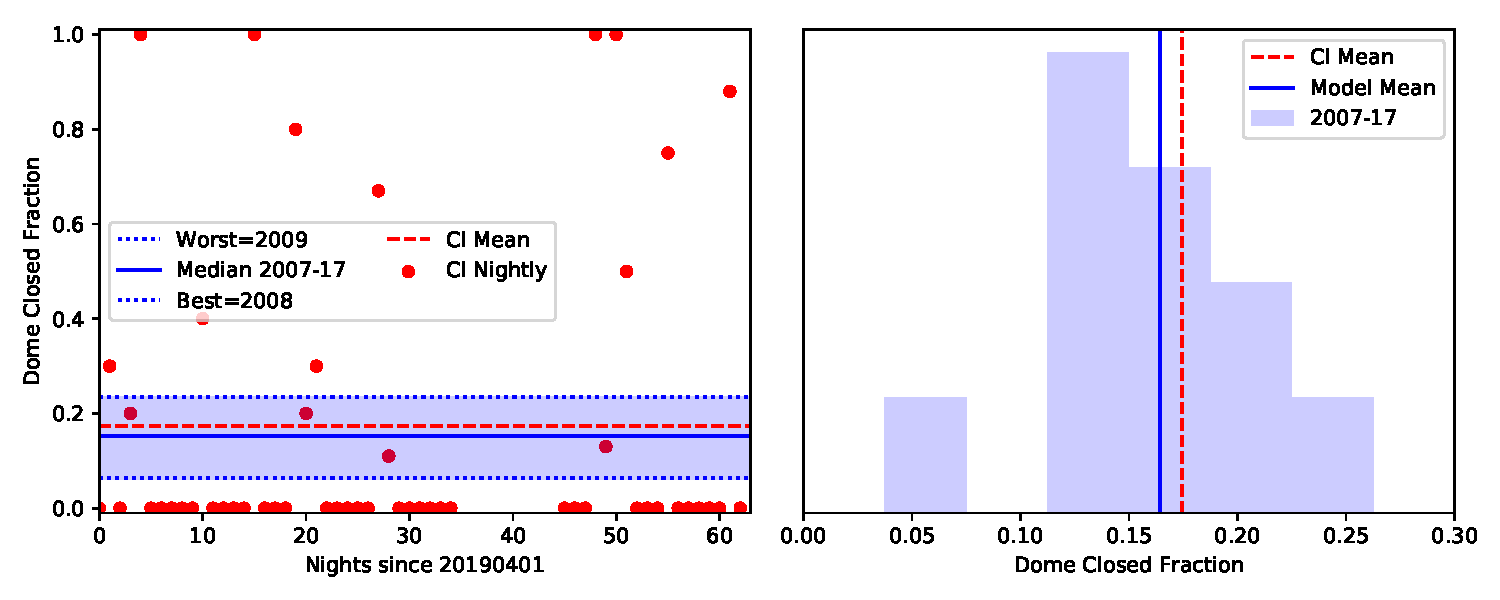
\includegraphics[width=6in]{CIdome}
\caption{Actual (red) and predicted (blue) dome-closed fraction for the dates corresponding to the CI run. The left hand plot
shows the time series of dome-closed fractions inferred from the night log, compared with the best, mean and worst years. The
shutdown period May 6 - 15 is omitted from both the actual and predicted calculations. The right-hand plot compares the actual
weather fraction with the distribution for the same dates in each of the years 2007-17.}
\label{fig:CIdome}
\end{center}
\end{figure}

\section{Delivered Image Quality}

To be completed in a future version of this document.

\section{Sky Transparency}

To be completed in a future version of this document.

\bibliographystyle{unsrt}
\bibliography{CommWeather}

\end{document}
